\documentclass{article}
\usepackage{graphicx}
\usepackage[textgreek}

\title{COMP26120 Lab 5}
\author{Michael Krasa}

\begin{document}
\maketitle

% PART 2 %%%%%%%%%%%%%%%%%%%%%%%%%%%%%%%%%%%%%%%%%%%%%%%%%%%%%%%%%%%%%%%%%%%%%%

\section{Complexity Analysis}
\label{sec:complexity}




\subsection{Insertion Sort}

Insertion sort is said to be very efficient for small data sets just like other quadratic sorting algorithms but gets seriously slow with larger arrays. Its worst case scenario is \Theta(n^2) comparisons and swaps. 

The insertion sort takes the maximum amount of time if elements are sorted in reverse order. In this case the inner loop will have to shift all the sorted section of the array before inserting with each iteration and when looking for its correct position the for loop also has to iterate throught the entire dictionary each time. This makes it very slow in cases where the dictionary is longer as an algorithm with quadratic time becomes slow very quickly. It is a stable sorting algorithm as it keeps the order of the elements it was given and doesn't reorder them during sorting.

It takes linear time \Theta(n) elements are already sorted. During each iteration the element is only compared with the high element and move onto the next one and finishes without any other nested loops which would increase the time taken.

Eventhough commenthing on the average case is beyond this course, I argue that given a random dictionary and queries the time should be close to \Theta(n^2). It is as the worst case scenario, since the algorithm has to do a lot of time-consuming comparing, swapping and most importantly the index changing for all elements with every single insertion, the only difference being that instead of searching all the way through the dictionary it might only need to go half way through it given that its an average case. For that very reason insertion sort is very useful when input array is almost sorted, only few elements are misplaced in complete big array.



\subsection{Quick Sort}

- Must define the recurrence equation and then solve it using something from the lecture

Quicksort is a divide and conquer algorithm, same as merge sort which we discussed in the lectures. It divides an array into two smaller sub-arrays. It can then sort the sub-arrays using recursion. 

We can write the time for the quick sort as following:
\begin{equation}
T(n) = T(k) + T(n-k-1) + \Theta(n)
\end{equation}
"T(k)" and "T(n-k-1)" are for two recursive calls and the last term is for the partition process. k represents the number of elements which are smaller than pivot in that recursive call. The time taken by quick sort depends on the input array (obviously) but also on partition strategy.

The best case occurs when the partition process always picks the median element as pivot. That way we would have two (near)equal lenght sub-arrays where the next pivot is easily determined. However, if a pivot isn't the median it doesn't mean that it will be that much slower, if at all. The time for the best case is \Theta(n log n).

T(n) = 2T(n/2) + \Theta(n)

The worst case occurs when the partition process picks the greatest or smallest element as pivot. If that were to happen the program would waste time by doing a an n number of passes before moving the pivot again. The time for that is \Theta(n^2).

T(n) = T(0) + T(n-1) + \Theta(n)

%====================================
\section{Experimental Analysis}
\label{sec:initialExperiments}

In this section we consider the question:
	\begin{quote}
	Under what conditions is it better to perform linear search rather than binary search?
	\end{quote}

\subsection{Experimental Design}

Before we design our experiment we have to keep several things in mind. First being the core difference between these two algorithms which is that binary search requires a sorted dictionary to perform as well as it does.

Knowing this, designing an experiment where this condition is true is quite simple. All we have to do is have an unsorted dictionary. This means that a binary search algorithm will have to sort the dictionary first which is time consuming, especially in larger dictionaries. We also have to decide on what sorting algorithm we'll use for the data set. Let's use quick sort because its best case scenario isn't necessarily an unprobable outlier and the algorithm can perform very close to it.

In this experiment we make the assumption that all the queries are in the dictionary, just to make the two algorithms a bit more closely matched.


\subsection{Experimental Results}

All we have to do now is put our two equations in a graphic calculator and see for ourselves. Since binary search is linear we do not need to include a sorting time complexity in its function, however, we have to do just that for the binary search, I am using the average case scenario which is usually very close to the worst case one.
Linear search complexity = \Theta(n)
Binary search complexity + quicksort = \Theta(n log n) + \Theta(log n)

\begin{figure}[h]
\caption{A comparison of the functions n log n + log n, and n}
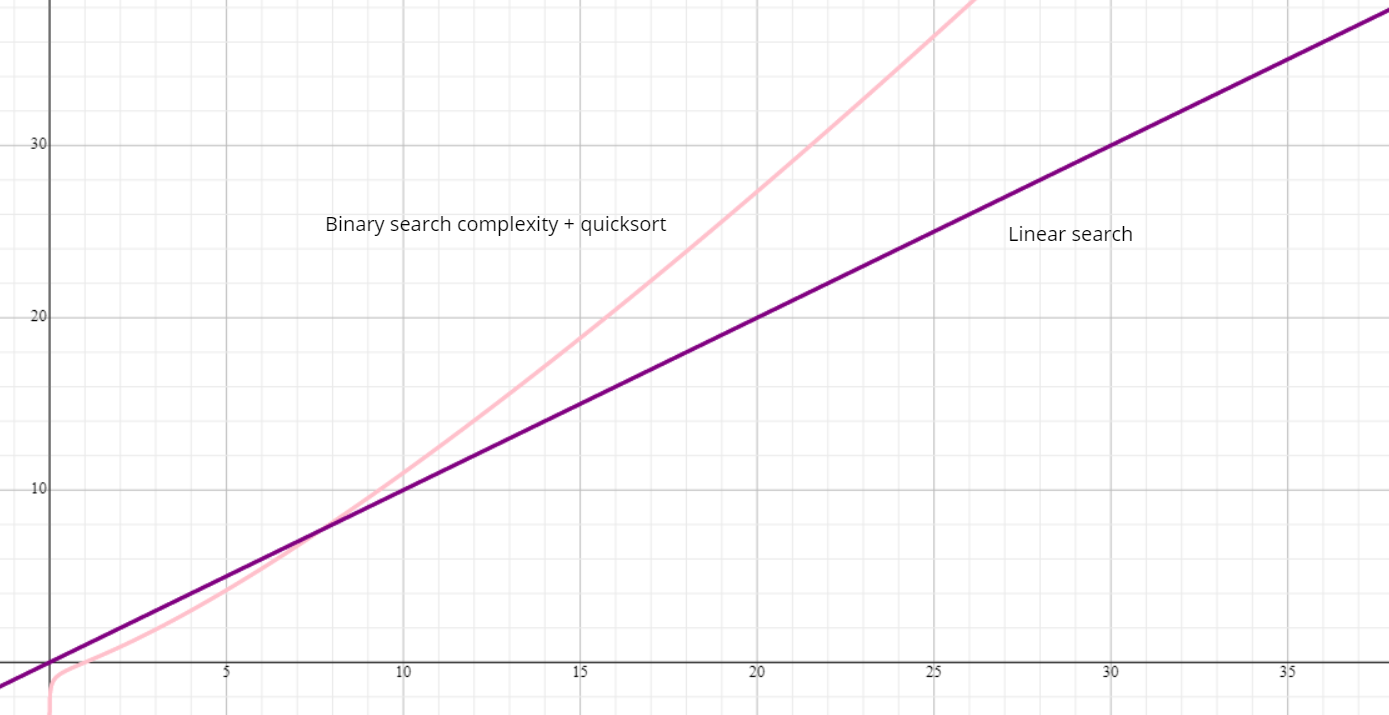
\includegraphics{graph1.png}
\centering
\end{figure}



Looking at figure 1 we can determine that given that the input is unsorted, it is better to use linear search for a dictionary that holds at least 5 elements. Since simply sorting the entire input alone would take longer than linear search a binary search approach is never the better option.


% PART 3 %%%%%%%%%%%%%%%%%%%%%%%%%%%%%%%%%%%%%%%%%%%%%%%%%%%%%%%%%%%%%%%%%%%%%%

\section{Extending Experiment to Data Structures}
\label{sec:part3}

We now extend our previously analysis to consider the question
\begin{quote}
Under what conditions are different implementations of the dictionary data structure preferable?
\end{quote}

% PART 3 %%%%%%%%%%%%%%%%%%%%%%%%%%%%%%%%%%%%%%%%%%%%%%%%%%%%%%%%%%%%%%%%%%%%%%
\section{Conclusions}
\label{sec:conclusions}
% Give your conclusions from the above experiments 


\end{document}
\documentclass{article}
\usepackage{graphicx}
\usepackage[textgreek}

\title{COMP26120 Lab 5}
\author{Michael Krasa}

\begin{document}
\maketitle

% PART 2 %%%%%%%%%%%%%%%%%%%%%%%%%%%%%%%%%%%%%%%%%%%%%%%%%%%%%%%%%%%%%%%%%%%%%%

\section{Complexity Analysis}
\label{sec:complexity}

- Worst, best - comment on average
- Mention that its data dependant
- Talk about some obscure scenarios - reverse sorted/already sorted


\subsection{Insertion Sort}

Insertion sort is said to be very efficient for small data sets just like other quadratic sorting algorithms but gets seriously slow with larger arrays. Its worst case scenario is \Theta (n^2) comparisons and swaps. 

The insertion sort takes the maximum amount of time if elements are sorted in reverse order. In this case the inner loop will have to shift all the sorted section of the array before inserting with each iteration. It is a stable sorting algorithm.

It takes minimum time \Theta (n) (linear time) when elements are already sorted. During each iteration the element is only compared with the high element and move onto the next one and finishes.

The average case is still \theta (n^2).  same as the worst case scenario, since the algorithm has to do a lot of time-consuming comparing, swapping and most importantly the index changing for all elements. For that very reason insertion sort is very useful when input array is almost sorted, only few elements are misplaced in complete big array. 



\subsection{Quick Sort}

- Must define the recurrence equation and then solve it using something from the lecture

Quicksort is a divide and conquer algorithm, same as merge sort which we discussed in the lectures. It divides an array into two smaller sub-arrays. It can then sort the sub-arrays using recursion. 

We can write the time for the quick sort as following:
\begin{equation}
T(n) = T(k) + T(n-k-1) + \Theta(n)
\end{equation}
"T(k)" and "T(n-k-1)" are for two recursive calls and the last term is for the partition process. k represents the number of elements which are smaller than pivot in that recursive call. The time taken by quick sort depends on the input array (obviously) but also on partition strategy.

The best case occurs when the partition process always picks the median element as pivot. That way we would have two (near)equal lenght sub-arrays where the next pivot is easily determined. However, if a pivot isn't the median it doesn't mean that it will be that much slower, if at all. The time for the best case is \Theta(n log n).

T(n) = 2T(n/2) + \Theta(n)

The worst case occurs when the partition process picks the greatest or smallest element as pivot. If that were to happen the program would waste time by doing a an n number of passes before moving the pivot again. The time for that is \Theta(n^2).

T(n) = T(0) + T(n-1) + \Theta(n)

%====================================
\section{Experimental Analysis}
\label{sec:initialExperiments}

In this section we consider the question:
	\begin{quote}
	Under what conditions is it better to perform linear search rather than binary search?
	\end{quote}

\subsection{Experimental Design}

Before we design our experiment we have to keep several things in mind. First being the core difference between these two algorithms which is that binary search requires a sorted dictionary to perform as well as it does.

Knowing this, designing an experiment where this condition is true is quite simple. All we have to do is have an unsorted dictionary. This means that a binary search algorithm will have to sort the dictionary first which is time consuming, especially in larger dictionaries. We also have to decide on what sorting algorithm we'll use for the data set. Let's use quick sort because its best case scenario isn't necessarily an unprobable outlier and the algorithm can perform very close to it.

In this experiment we make the assumption that all the queries are in the dictionary, just to make the two algorithms a bit more closely matched.


\subsection{Experimental Results}

All we have to do now is put our two equations in a graphic calculator and see for ourselves. Since binary search is linear we do not need to include a sorting time complexity in its function, however, we have to do just that for the binary search, I am using the average case scenario which is usually very close to the worst case one.
Linear search complexity = \Theta(n)
Binary search complexity + quicksort = \Theta(n log n) + \Theta(log n)

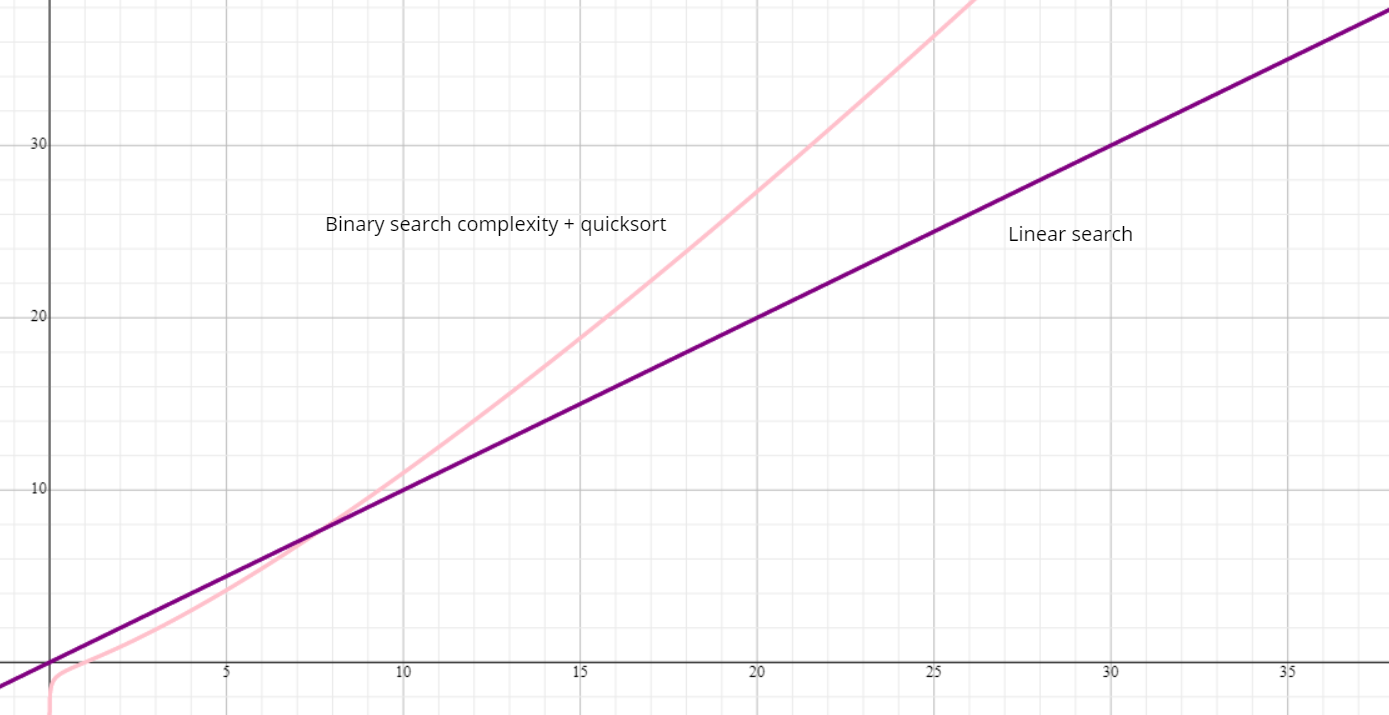
\includegraphics{graph1.png}



Looking at figure 1 we can determine that given that the input is unsorted, it is better to use linear search for a dictionary that holds at least 5 elements. Since simply sorting the entire input alone would take longer than linear search a binary search approach is never the better option.


% PART 3 %%%%%%%%%%%%%%%%%%%%%%%%%%%%%%%%%%%%%%%%%%%%%%%%%%%%%%%%%%%%%%%%%%%%%%

\section{Extending Experiment to Data Structures}
\label{sec:part3}

We now extend our previously analysis to consider the question
\begin{quote}
Under what conditions are different implementations of the dictionary data structure preferable?
\end{quote}

% PART 3 %%%%%%%%%%%%%%%%%%%%%%%%%%%%%%%%%%%%%%%%%%%%%%%%%%%%%%%%%%%%%%%%%%%%%%
\section{Conclusions}
\label{sec:conclusions}
% Give your conclusions from the above experiments 


\end{document}

